\tikzset{component/.style={draw, text width=2.5cm, align=center, minimum height=0.5cm}}
\tikzset{module/.style={draw, text width=0.75cm, align=center, minimum height=0.5cm}}

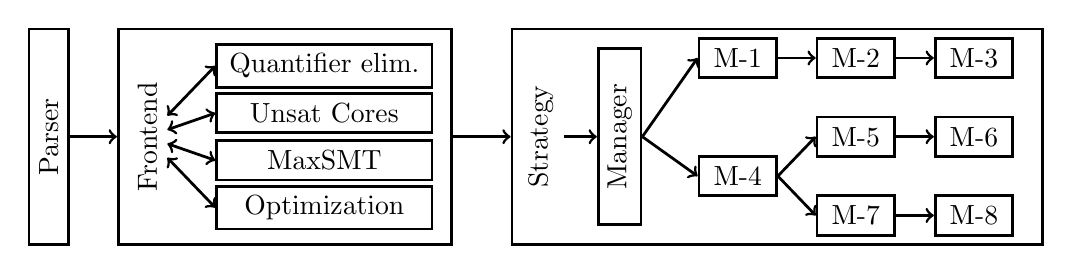
\begin{tikzpicture}[line width=1pt]

	\node[component, rotate=90] (parser) at (-0.25,0) {Parser};

	\node[component, text height=4cm, rotate=90] (frontend-box) at (2.75,0) {};
	\node[rotate=90] (frontend) at (1,0) {Frontend};

	\node[component] (optimization) at (3.25,-0.9) {Optimization};
	\node[component] (maxsmt) at (3.25,-0.3) {MaxSMT};
	\node[component] (unsat-cores) at (3.25,0.3) {Unsat Cores};
	\node[component] (qe) at (3.25,0.9) {Quantifier elim.};

	
	\node[component, text height=6.5cm, rotate=90] (strategy-box) at (9,0) {};
	\node[rotate=90] (strategy) at (6,0) {Strategy};
	\node[component, text width=2cm, rotate=90] (manager) at (7,0) {Manager};

	\node[module] (module1) at (8.5,1) {M-1};
	\node[module] (module2) at (10,1) {M-2};
	\node[module] (module3) at (11.5,1) {M-3};
	\node[module] (module4) at (8.5,-0.5) {M-4};
	\node[module] (module5) at (10,0) {M-5};
	\node[module] (module6) at (11.5,0) {M-6};
	\node[module] (module7) at (10,-1) {M-7};
	\node[module] (module8) at (11.5,-1) {M-8};
	

	\draw[->] (parser) -- (frontend-box);
	\draw[->] (frontend-box) -- (strategy-box);
	\draw[->] (strategy) -- (manager);
	\draw[<->] (frontend) -- (qe.west);
	\draw[<->] (frontend) -- (unsat-cores.west);
	\draw[<->] (frontend) -- (maxsmt.west);
	\draw[<->] (frontend) -- (optimization.west);

	\draw[->] (manager.south) -- (module1.west);
	\draw[->] (module1.east) -- (module2.west);
	\draw[->] (module2.east) -- (module3.west);
	\draw[->] (manager.south) -- (module4.west);
	\draw[->] (module4.east) -- (module5.west);
	\draw[->] (module4.east) -- (module7.west);
	\draw[->] (module5.east) -- (module6.west);
	\draw[->] (module7.east) -- (module8.west);
\end{tikzpicture}